	
\chapter{CNN test for MNIST}	
	
	\section{Benchmark Dataset}
	\subsection{MNIST}
	The MNIST database of handwritten digits, has a training set of 60,000 examples, and a test set of 10,000 examples. It is a subset of a larger set available from NIST. The digits have been size-normalized and centered in a fixed-size image. Each example is a $28\times 28$ grey-scale image with a label that show witch number the image is.
%	\subsection{to be continued}




	\section{The math representation of data and function}
	Let $\mathcal{M}$ is the number of examples in training data, $\mathcal{C}$ is the number of the variety of label.
	
	\subsection{Label} Each image has a label in $\{0,1,\cdots,9\}$ to show what's the number it is. We transform the label $n$ to a 10-dimension vector which the $n$-th element is $1$ and others are $0$, i.e. 
	$$
	n \rightarrow \mathbf y
	$$
	where $y_i = 1 $ iff $i=n$.
	Then the label data can be present as a matrix $Y = (\mathbf y_1,\cdot,\mathbf{y}_{\mathcal M})$.
	\subsection{Grey-scale Image}
	In this note, we only focus on the CNN of 2D image. A 2D Grey-scal image can regard as a matrix $X =(x_{m,n})_{M\times N}$ where $x_{m,n}$ is the grey-level of pixel $(m,n)$.
	\subsection{Image with multiple channels}
	If we put more than one value on each pixel, the image can be think as a 3-rank tensor $\mathbf X = (x_{m,n,l})_{M\times N\times L}$ which $x_{m,n,l}$ is the $l$-th value on pixel $(m,n)$. For example, a colorful image usually has three channels: red, blue and green. More over, we can consider that a channel is a feature of the image, so we usually create more channels in the convolution layer so that we can get more features.
%	\subsection{Data between two layer}
%	The transport data $\mathbf X$ between two layer can be describe as a 3-rank tensor, i.e. $\mathbf X = (x_{m,n,l})_{M\times N\times L}$. We can regard it as a 2D image with L real number in each pixel.
	\subsection{Convolution Kernel}
	A 2D-convolution kernel for a 2D image can be represent as a matrix, i.e. $K = (k_{i,j})_{I\times J}, i= -I',-I'+1,...,I', j = -J',-J'+1,...,J'$.(Suppose $I$ and $J$ is odd integer and $I' = \dfrac{I-1}2, J' = \dfrac{J-1}2 $.) which $K_{i,j}$ is the parameter on pixel $(i,j)$.
	
	The effect of a $I\times J$ kernel $K$ acting on a $M\times N$  image $X$ is a 2D image 
	$$
	Y =	 K ( X) = (y_{m,n})_{M\times N}
	$$
	where 
	\begin{equation}
	y_{m,n} =\sum_{\alpha = - I'}^{I'} \sum_{\beta = - J'}^{J'}k_{\alpha,\beta} x_{m+\alpha,n+\beta}
	\end{equation}
	
	A 2D-convolution kernel for a 2D image with $L$ channels can be represent as a 3-rank tensor, i.e. $\mathbf{K} = (k_{i,j,l})_{I\times J\times L}, i= -I',-I'+1,...,I', j = -J',-J'+1,...,J'$.(Suppose $I$ and $J$ is odd integer and $I' = \dfrac{I-1}2, J' = \dfrac{J-1}2 $.) which $K_{i,j,l}$ is the parameter of $l$-th channel on pixel $(i,j)$.
	
	 The effect of a $I\times J\times L$ kernel $\mathbf K $ acting on a $M\times N \times L$ multiple channel image $\mathbf X$ is also a 2D image 
	$$
		Y =	\mathbf K (\mathbf X) = (y_{m,n})_{M\times N}
	$$
	where 
	\begin{equation}
	y_{m,n} =\sum_{l=1}^L\sum_{\alpha = - I'}^{I'} \sum_{\beta = - J'}^{J'}k_{\alpha,\beta,l} x_{m+\alpha,n+\beta,l}
	\end{equation}
	
	 A convolution layer usually has more than one kernels, if we write them together, we can get a 4-rank tensor $\mathcal{K} = (k_{i,j,l,p})_{I\times J\times L\times P}$ where $\mathbf K_p = (k_{i,j,l,p})_{I\times J\times L}$ is the $p$-th kernel.
	Then we can easily get the effect of a $I\times J\times L\times P$ kernel $\mathcal K $ acting on a $M\times N \times L$ multiple channel image $\mathbf X$ is a 2D image with $P$ channels
	$$
	\mathbf Y =	\mathcal K (\mathbf X) = (y_{m,n,p})_{M\times N\times P}
	$$
	where 
	\begin{equation}
	y_{m,n,p} =\sum_{l=1}^L\sum_{\alpha = - I'}^{I'} \sum_{\beta = - J'}^{J'}k_{\alpha,\beta,l,p} x_{m+\alpha,n+\beta,l}
	\end{equation}
	\subsection{Pooling function}
	Suppose $X$ is a $S \times T$ matrix, we have pooling function:
	\begin{itemize}
		\item max-pooling: 
		$$
			P^{max}_{S\times T}(X) = \max x_{s,t}
		$$
		\item mean-pooling:
		$$
		P^{mean}_{S\times T}(X) = \dfrac 1{ST} \sum_{s,t}x_{s,t}
		$$
	\end{itemize}
	Now let X is a $M \times N$ matrix and $M=S\times A, N=T\times B$, we write $X$ in block matrix
	\begin{equation}
	X=\left[
	\begin{matrix}
	X_{1,1}&\cdots	&X_{1,B}\\
	\vdots &	  	&\vdots\\
	X_{A,1}&\cdots	&X_{A,B}
	\end{matrix}
	\right]
	\end{equation}. Each block $X_{a,b}$ is a $S\times T$ matrix.
	
	After we selected a pooling function $P_{S\times T}$, then 
	$$
		Y = P_{S\times T}(X) =(y_{a,b})_{A\times B}
	$$
	where
	\begin{equation}
	 y_{a,b} = P_{S\times T}(X_{a,b})
	\end{equation}
	
	\subsection{Loss function}\label{Loss}
	\paragraph{Cross-entropy} Suppose $\mathbf y$ is the training data transformed by a example's label and $\hat {\mathbf {y}}$ is calculate by our model, the cross-entropy loss function is:
	\begin{equation}
	L(\mathbf y,\hat {\mathbf {y}}) =- \sum y_n \ln \hat{y}_n
	\end{equation}
	
	So the loss function of training data is 
	\begin{equation}
	\mathcal L(Y,\hat Y) = \sum L(\mathbf y_i,\hat {\mathbf {y}}_i)
	\end{equation}
	
 	\section{Introduction of several kinds of Layer}
	\subsection{Densely Connect Layer}\label{Dense}
	This kind of layer is same with DNN. The input is a vector $\mathbf x$ and the parameter is a matrix $W$ and vector $\mathbf b$ called bias. After we choose a active function $\sigma$, the output is
	\begin{equation}
	\mathbf u = \sigma(W \mathbf x + \mathbf b)
	\end{equation}
	\subsection{Convolution Layer}\label{Convolution}
	Suppose input data is a $M \times N \times L $ multi-channel image $\mathbf X$. Parameter of this layer is a $I\times J\times L\times P$ tensor $\mathcal K$ and a P-dimension vector $\mathbf b = (b_1,...,b_p)$ called bias. After we choose a active function $\sigma$. Then the output of this layer is a $M\times N \times P$ tensor  
	$$
		\mathbf U = \sigma(\mathcal{K}(\mathbf X) + \mathbf B)
	$$
	where $\mathbf B =(B_{m,n,p})_{M\times N\times P}$ and $B_{m,n,p} = b_p$ 
	\subsection{Pooling Layer}\label{Pooling}
	Suppose input data is a $M \times N \times L $ multi-channel image $\mathbf X$ and $M=S\times A, N=T\times B$. The $l$-th channel of $X$ is a $M\times N$ matrix $X_p$. The output of this layer is a $A\times B\times P$ multi-channel image:
	
	$$
	\mathbf U =P_{S\times T}(\mathbf X)=(U_p)_{P}
	$$
	where 
	\begin{equation}
	U_p = P_{S\times T}(X_p)
	\end{equation}
	\subsection{Dropout Layer}\label{Dropout}
	For a input $N$-element vector $\mathbf x$, and a number $\gamma \in [0,1]$, the output is 
	$$
	\mathbf u = (u_n)_N = \text{dropout}_{\gamma} (\mathbf x)
	$$
	where 
	\begin{equation}
	u_n = \left \{ 
	\begin{split}
	x_n &\ \text{with probility}\ \gamma\\
	0   &\ \text{with probility}\ 1-\gamma
	\end{split}
	\right.
	\end{equation}
	\subsection{Classifier Layer}
	\paragraph{Softmax Classifier}\label{Softmax} For a input vector $x$ and the parameter is a matrix $W$ and vector $\mathbf b$ called bias. Then 
	$$
	\mathbf y = W\mathbf x + \mathbf b 
	$$
	and the output is 
	\begin{equation}
		\mathbf u = (u_c)_{\mathcal C} =\text{softmax}(\mathbf y)
	\end{equation}
	where 
	\begin{equation}
	u_c = \dfrac{e^{y_c}}{\sum_{c=1}^{\mathcal{C}} e^{y_c}}
	\end{equation}
\iffalse
	\begin{table}[h]
		\begin{tabular}{ccc}
			Kind of Layer &\\ \hline
			Convolution Layer 		&\\
			Pooling Layer 			&\\
			Densely Connected Layer &\\
			Dropout Layer			&\\
			Classifier Layer		&\\
		\end{tabular}
	\end{table}
\fi
	\section{A Example of CNN}
	This CNN totally contains 7 hidden layers. The describe of each layer is listed in follow table.
	\newpage
	\begin{table}
		\begin{tabular}{|c|c|c|}\hline
		Layer 						&Input and			&Output	\\
									&Parameter			&\\ \hline
		0 Input Layer    			& 					& $X[28,28]$\\\hline
		1 Convolution Layer 		&$\mathbf X[28,28,1] = X$			&$\mathbf U_1[28,28,32]$\\
        &$\mathcal K_1[5,5,1,32], \mathbf b_1[32]$	&$\mathbf U_1 = \sigma (\mathcal K_1(\mathbf X)+ \mathbf B_1)$ (\ref{Convolution})\\\hline
		2 Pooling Layer 			&$\mathbf U_1[28,28,32]$	&$\mathbf U_2[14,14,32]$\\
		&							&$\mathbf U_2 = P_{2\times 2}^{\max}(\mathbf U_1)$ (\ref{Pooling})\\\hline
		3 Convolution Layer			&$\mathbf U_2$[14,14,32]		&$\mathbf U_3[14,14,64]$\\
		&$\mathcal K_2[5,5,32,64], \mathbf b_2[64]$&$\mathbf U_3 = \sigma (\mathcal K_2(\mathbf U_3)+ \mathbf B_2)$(\ref{Convolution})\\	\hline
		4 Pooling Layer 			&$\mathbf U_3[14,14,64]$		&$\mathbf U_4[7,7,64]$\\
		& 							&$\mathbf U_4 = P_{2\times 2}^{\max}(\mathbf U_3)$(\ref{Pooling})\\\hline
		5 Densely Connected Layer 	&$\mathbf x[3136] = \text{vec}(\mathbf U_4)$ &$\mathbf u_1[1024]$\\
		&$W[3136,1024],\mathbf b[1024]$		&$\mathbf u_1 = \sigma (W\mathbf x +\mathbf b)$(\ref{Dense})\\\hline
		6 Dropout Layer				&$\mathbf u_1[1024]$ 				&$\mathbf u_2[1024]$\\
		(Only be used in training)&					&$\mathbf u_2 = \text{dropout}_{0.5}(\mathbf u_1)$(\ref{Dropout})\\\hline
		7 Softmax Layer				&$\mathbf u_2[1024]$				&$\hat{\mathbf y}[10]$\\
		&$W_s[1024,10],\mathbf b_s[10]$	&$\hat{\mathbf y} = \text{softmax}(W_s\mathbf x +\mathbf b_s)$(\ref{Softmax}) \\\hline
		8 Output Layer				&									&\\ \hline
		\end{tabular}
	\end{table}
	
	In this table $\mathbf X[a,b,c]$ means $\mathbf X$ is a $a\times b\times c$ tensor.
\iffalse
	\begin{table}
	\begin{tabular}{ccc}
		Layer or Output & &Detail\\ \hline
	Layer 0 & Input a picture $\mathbf x$& $\mathbf x$ is a 28$\times$28 matrix \\\hline
	Layer 1 & Convolution Layer 		& \\
	Output of Layer 1 &  		&$\mathbf{u}_1$ is a 28$\times$28$\times$32 tensor\\ \hline
	Layer 2 & Pooling Layer 			&\\
	Output of Layer 2 &  		&$\mathbf{u}_2$ is a 14$\times$14$\times$32 tensor\\ \hline
		3 & Convolution Layer		&\\
	Output of Layer 3 &  		&$\mathbf{u}_3$ is a 14$\times$14$\times$64 tensor\\ \hline
		4 & Pooling Layer 			&\\
	Output of Layre 4&&$\mathbf{u}_4$ is a 7$\times$7$\times$64 tensor\\\hline
		5 & Densely Connected Layer &\\
	Output of Layer 5 &  		&$\mathbf{u}_5$ is a 1024 vector\\ \hline
		6 & Dropout Layer			&\\
	Output of Layer 6 &  		&$\mathbf{u}_6$ is a 1024 vector\\ \hline
		7 & Softmax Layer			&\\
	Output of Layer 5 &  		&$\mathbf{y}$ is a 10 vector\\ \hline
		8 & Output Layer			&output $\mathbf{y}$\\ 
	
	\end{tabular}
\end{table}
\fi
	
	\section{Optimizer and Numerical Result} 
	For a input image $X_m$ in training data, now we can get $\hat{\mathbf y}_m = \hat{\mathbf y}(X_m,\bm \theta)$, where $\bm \theta = (\mathcal K_1, \mathbf b_1,\mathcal K_2, \mathbf b_2,W,\mathbf b,W_s,\mathbf b_s)$, Let $\hat{Y} = (\hat{\mathbf y}_1,\cdots,\hat{\mathbf y}_{\mathcal{M}})$
	Now we get the optimize question: Find 
	$\bm \theta$ s.t.
	$$
	 \min	\mathcal{L}(Y,\hat{Y}) = \sum_{m=1}^{\mathcal M} L(\mathbf y_m, \hat{\mathbf{y}}_m)
	$$
	($L$ is in \ref{Loss}).
	
	The optimizers for this question is the same as optimizers in DNN. The numerical result of this CNN is showing below: The first figure show the accuracy rate, second figure is the value of loss function $\mathcal L$ and the third figure show the value of $-\lg \mathcal{L}$. Besides. 
	
\begin{figure}
	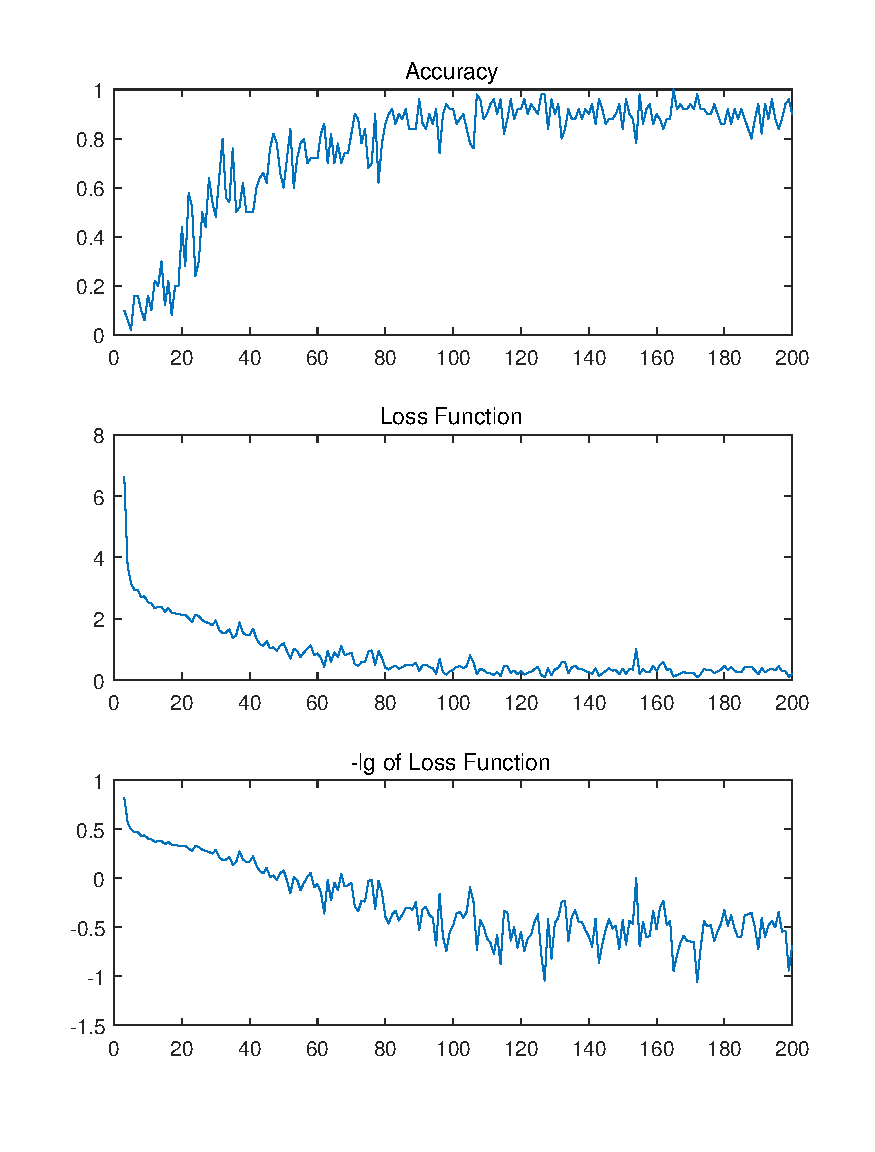
\includegraphics[width = \textwidth,height=0.5\textheight]{SGD_relu_200}
	\caption{ Active function is relu, algorithm is SGD, step = 200,learning rate is 0.1}
	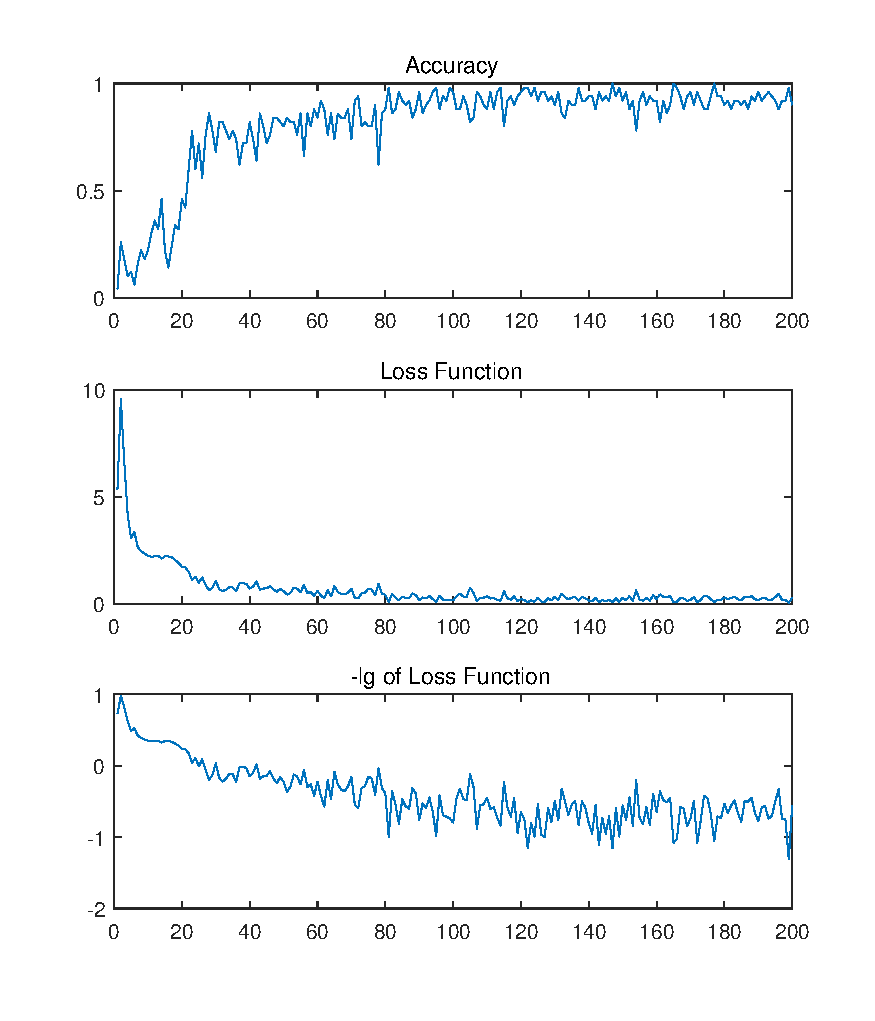
\includegraphics[width = \textwidth,height=0.5\textheight]{Momentum_relu_200}
	\caption{active function is relu, algorithm is Momentum, step = 200, learning rate is 0.03, momentum rate is 0.9}
\end{figure}

\begin{figure}
	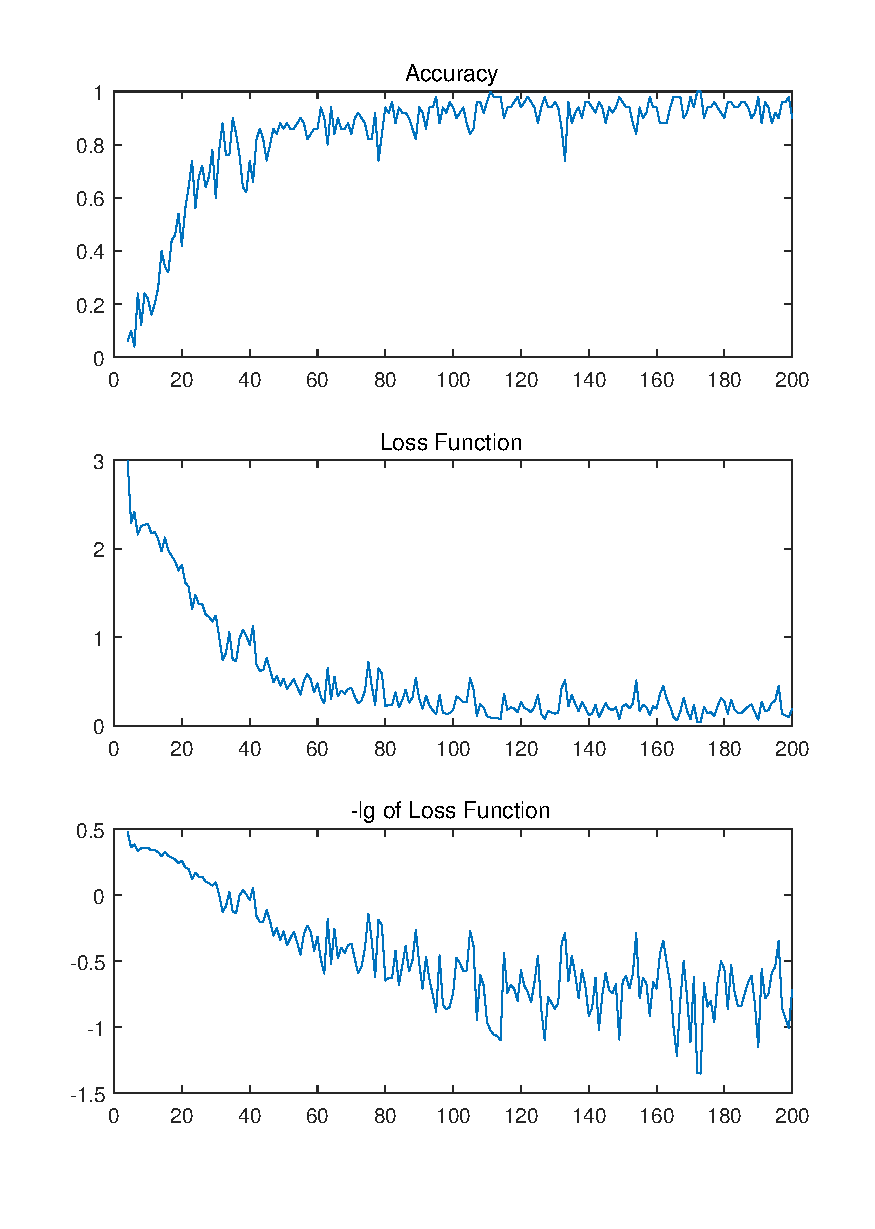
\includegraphics[width = \textwidth,height=0.5\textheight]{Adagrad_relu_200}
	\caption{ Active function is relu, algorithm is Adagrad, step = 200,learning rate is 0.1}
	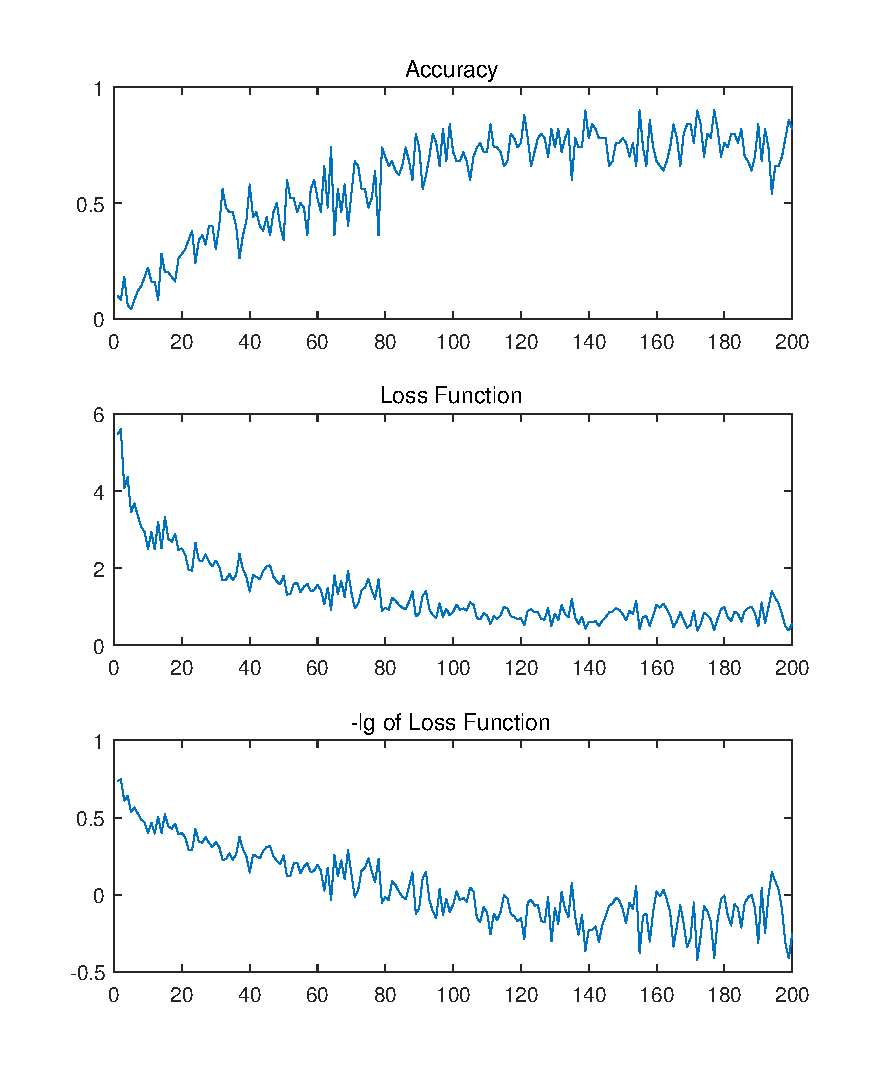
\includegraphics[width = \textwidth,height=0.5\textheight]{Adadelta_relu_200}
	\caption{active function is relu, algorithm is Adadelta, step = 200,learning rate is 0.1}
\end{figure}
\begin{figure}
	
	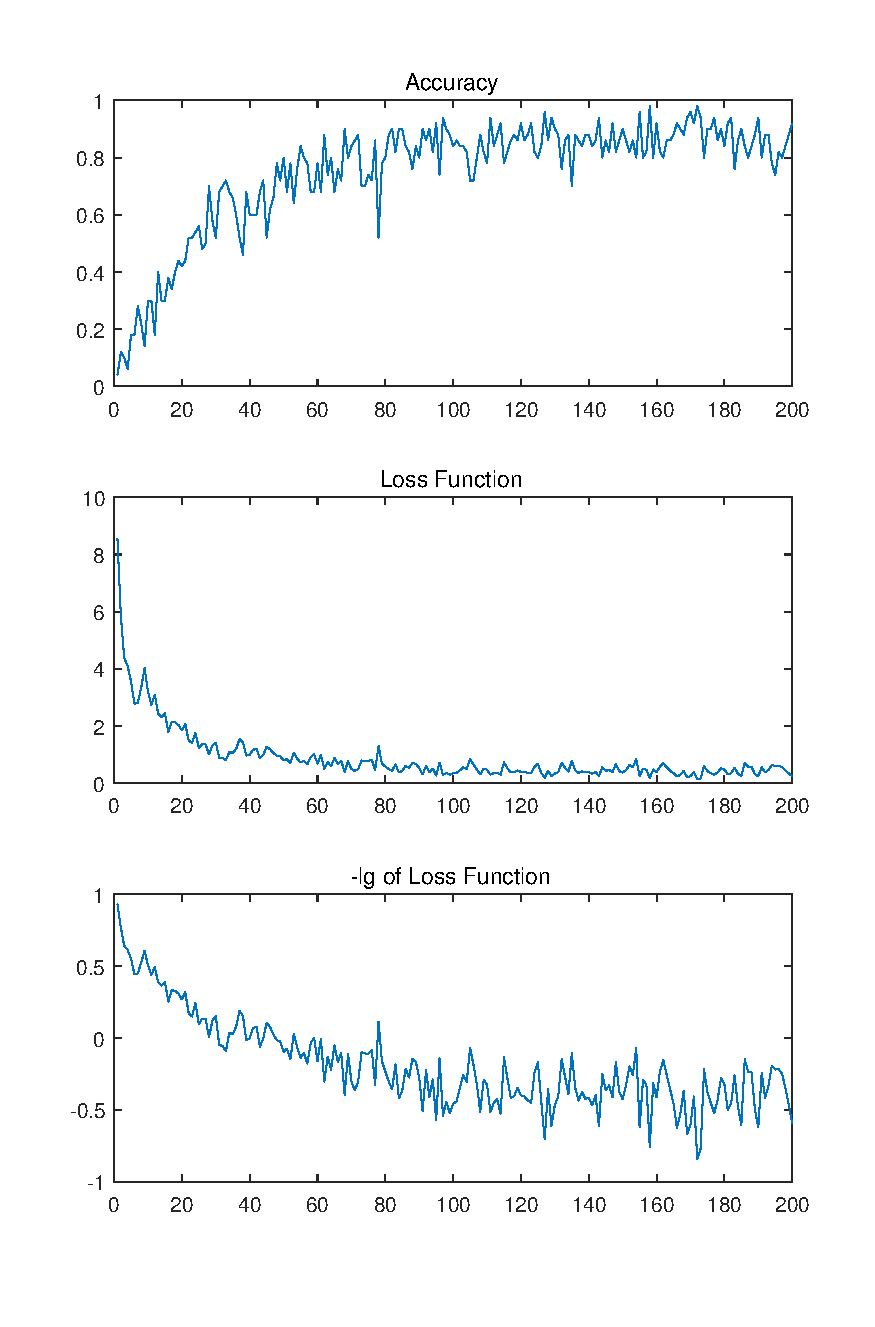
\includegraphics[width = \textwidth,height=0.5\textheight]{Adam_relu_200}
	\caption{active function is relu, algorithm is Adam, step = 200,learning rate is 0.0001 }
\end{figure}

\subsection{Logistic regression }
\subsubsection{Model}
\begin{itemize}
\item X: the input image of a handwritten digit
\item Y: the true value of the digit
\item W,b: weight and bias
\item Y$\_$pred=softmax(Wx+b)
\item Loss=cross$\_$entropy(Y, Y$\_$pred)+ regularization term
\item Optimization method: Adam
\end{itemize}

\subsubsection{Implementation }
\begin{itemize}
\item Parameter
\begin{enumerate}
\item learning rate = 0.001
\item training epochs=50
\item batch size =100
\item regularization coefficient =0.0001
\end{enumerate}
\item Result
\begin{enumerate}
\item no regularization: training accuracy=93$\%$; test accuracy =92$\%$
\item regularization coefficient =0.0001: training accuracy=93$\%$; test accuracy =92$\%$
\item regularization coefficient =0.001: training accuracy=92$\%$; test accuracy =92$\%$
\item no regularization+SGD: training accuracy= 88$\%$; test accuracy =89$\%$
\end{enumerate}

\end{itemize}

\subsection{One hidden layer }
\subsubsection{Model}
\begin{itemize}
\item X: the input image of a handwritten digit
\item Y: the true value of the digit
\item Hidden layer size=500
\item Loss=cross$\_$entropy(Y, Y$\_$pred)+ regularization term
\item Optimization method: Adam
\end{itemize}

\subsubsection{Implementation }
\begin{itemize}
\item Parameter
\begin{enumerate}
\item learning rate = 0.001
\item training epochs=50
\item batch size =100
\item regularization coefficient =0.0001
\end{enumerate}
\item Result
\begin{enumerate}
\item no regularization: training accuracy=100$\%$; test accuracy =98.36$\%$
\item regularization coefficient =0.0001: training accuracy=99.00$\%$; test accuracy =98.04$\%$
\item regularization coefficient =0.001: training accuracy=98.00$\%$; test accuracy =97.67$\%$
\item no regularization+SGD: training accuracy= 90$\%$; test accuracy =90.54$\%$
\end{enumerate}

\end{itemize}


\section{MgNet and iResNet results}
\subsection{MgNet}
\begin{description}
	\item[Model] The hyperparameters:
\begin{itemize}
	\item $J$: the number of grids. we choose $J = 4$, that makes $m_4 = n_4 = 5$.
	\item $\nu_\ell$:  the number of smoothings in each grids, 
	just take $\nu_\ell = 2$.
	\item $c_u=c_f = 64$: the number of feature and data channels. 
	\item $A^\ell = \xi^{\ell} $ and $B_{\ell,i} = \sigma \circ \eta^{\ell,i} \circ \sigma $ are all convolution with multichannel with 
	$\mathbb{R}^{3\times3\times c\times c}$
	which need to be trained.
	\item $R_{\ell}^{\ell+1}$ and $\Pi_{\ell}^{\ell+1}$: the interpolation 
	and restriction operator in MgNet.  
	Here we choose it as a convolution with stride $2$ which need to be trained.
\end{itemize}

\item[Result] The result is: \\
model size: 557514, acc: 99.56, acc best: 99.60

\end{description}

\subsection{iResNet}
\begin{description}
	\item[Model] The hyperparameters:
	\begin{itemize}
	\item $J$: the number of grids. we choose $J = 4$, that makes $m_4 = n_4 = 5$.
\item $\nu_\ell$:  the number of smoothings in each grids, 
in iResNet, because of the definition of $f^{\ell+1,0}$, so $(\nu_1, \cdots, \nu_{4}) = (2,1,1,1)$.
\item $c_f$: the number of channels.  Some suggestions:
\blue{\begin{itemize}
		\item The original iResNet-18: $(c_{f,1}, \cdots, c_{f,4}) = (64,128,256,512)$, but too many parameters.
		\item You can try $(16,32, 64, 128)$, less parameters.
		\item You can also try $(64,64,64,64)$, or any set up for channels.
\end{itemize}}
\item $\xi^{\ell,i} $ and $\eta^{\ell,i} $ are all convolution with multichannel with 
$\mathbb{R}^{3\times3\times c\times c}$
which need to be trained.
\item $R_{\ell}^{\ell+1}$ and $\eta^{\ell,0}$: the restriction operator. 
Here we choose it as a convolution with stride $2$ which need to be trained.
	\end{itemize}
	
	\item[Result] The result for $(16,32, 64, 128)$ is: \\
	model size: 605898,  acc: 99.52,  acc best : 99.56.
	
\end{description}